\documentclass[11pt,a4paper]{article}
\usepackage[a4paper,left=22mm,right=22mm,bottom=22mm,top=22mm]{geometry}
\usepackage{fontspec}
\usepackage[british]{babel}
\usepackage{amsmath,amssymb,graphicx,booktabs,array,tabularx,fancyhdr}
\usepackage[square,comma,numbers,sort&compress]{natbib}
\usepackage[hidelinks]{hyperref}
\usepackage{caption,subcaption}
\usepackage{float}
\usepackage{placeins}
\usepackage{microtype}
\usepackage{xcolor}
\usepackage{algorithm}
\usepackage{algpseudocode}
\graphicspath{{figures/}}
\captionsetup{font=small,labelfont=bf}
\setlength{\parindent}{0em}
\setlength{\parskip}{0.4em}
\setlength{\headheight}{14pt}
\renewcommand{\topfraction}{0.9}
\renewcommand{\textfraction}{0.07}
\renewcommand{\floatpagefraction}{0.8}
\renewcommand{\bottomfraction}{0.8}
\setcounter{topnumber}{3}
\setcounter{bottomnumber}{3}
\setcounter{totalnumber}{5}
\pagestyle{fancy}
\fancyhead{}
\fancyhead[C]{\small Lab 6: Two-view geometry and motion estimation}
\fancyfoot{}
\fancyfoot[C]{\thepage}
\renewcommand{\headrulewidth}{0pt}
\renewcommand{\abstractname}{Summary}
\newcommand{\studentname}{Team Fullcans}
\DeclareRobustCommand{\code}[1]{\begingroup\ttfamily\codebreaks#1\endgroup}
\newcommand{\codebreaks}{\renewcommand{\_}{\textunderscore\allowbreak}}
\newcommand{\skewm}[1]{[#1]_{\times}}
\setlength{\emergencystretch}{3em}
\title{Lab 6 Report\\[0.3em]\large Minimal solvers, RANSAC and frame-to-frame motion estimation}
\author{\studentname}
\date{Report date: 10 November 2026}
\hypersetup{pdftitle={Lab 6 Report: Two-view geometry and motion estimation}}

\begin{document}
\maketitle

\begin{abstract}
Frame-to-frame motion estimation must recover the camera pose from feature matches
that contain outliers. We derive the minimal solvers behind this task, Nist\'er's
five-point algorithm and a two-point solver for known rotation, together with the
RANSAC iteration counts they imply. We then evaluate four solvers inside RANSAC on all
3\,887 consecutive frame pairs of a simulated office flight. A sub-pixel inlier
threshold of 0.1\,px brings the five-point solver to a median rotation error of
0.034$^\circ$, ten times lower than at 1\,px. Prior information gives the largest
further gain. A known rotation lowers the median translation-direction error from
0.066 to 0.020 at 0.39\,ms per frame, and depth lets Arun's 3D--3D method reach
0.019$^\circ$ and 1.7\,mm. Without RANSAC, the same matches give rotation errors of
0.6--14$^\circ$.
\end{abstract}

\section{Individual work}

\paragraph{Notation.}
Two calibrated views are taken at times $t_1$ and $t_2$. A correspondence is a pair of
unit bearing vectors $(f_1, f_2)$ that point to the same 3D point from the two camera
centres. The relative pose $(R, t)$ maps coordinates in frame 2 to frame 1,
$p_1 = R p_2 + t$: $R$ rotates frame 2 into frame 1, and $t$ is the centre of camera 2
expressed in frame 1. Since $\lambda_1 f_1 = \lambda_2 R f_2 + t$, the vectors $f_1$,
$R f_2$ and $t$ are coplanar, which gives the epipolar constraint
\begin{equation}
  f_1^\top E f_2 = 0, \qquad E = \skewm{t} R .
  \label{eq:epipolar}
\end{equation}
OpenGV~\cite{kneip2014opengv}, used in the team part, follows the same convention.

\subsection{Deliverable 1: Nist\'er's five-point algorithm}

\paragraph{1. Computational steps.}
Nist\'er's solver~\cite{nister2003efficient} takes five correspondences and returns
every essential matrix consistent with them, at most ten, each with its pose $(R, t)$
up to scale.
\begin{enumerate}
  \item \emph{Null space of the linear constraints.} With $E$ stored row by row as
    $\tilde E \in \mathbb{R}^9$, each correspondence turns \eqref{eq:epipolar} into
    $(f_1 \otimes f_2)^\top \tilde E = 0$. Five correspondences give a $5\times 9$
    matrix with a four-dimensional null space. Its basis $X, Y, Z, W$ (from QR or SVD)
    parametrises every candidate as $E = xX + yY + zZ + W$.
  \item \emph{Cubic constraints.} A valid essential matrix has two equal singular
    values and one zero singular value, which is equivalent to
    \begin{equation}
      \det E = 0, \qquad 2EE^\top E - \operatorname{tr}(EE^\top)E = 0 .
      \label{eq:cubic}
    \end{equation}
    Substituting the parametrisation gives ten cubic equations in $(x,y,z)$, written
    as a $10\times 20$ matrix over the 20 monomials of degree at most 3.
  \item \emph{Gauss--Jordan elimination.} Eliminating this matrix with a suitable
    monomial order leaves rows that Nist\'er combines into three polynomials
    $\langle k\rangle$, $\langle l\rangle$ and $\langle m\rangle$. Together they form a
    $3\times 3$ matrix $B(z)$, polynomial in $z$, with $B(z)\,[x\ y\ 1]^\top = 0$.
  \item \emph{Tenth-degree polynomial.} A non-trivial solution requires
    $\det B(z) = 0$, a univariate polynomial of degree 10. Its real roots are
    bracketed with a Sturm sequence and refined by bisection or Newton steps.
  \item \emph{Back-substitution.} For each real root $z$, the null vector of $B(z)$
    gives $(x, y)$, and hence $E = xX + yY + zZ + W$.
  \item \emph{Pose recovery.} The SVD $E = U\operatorname{diag}(1,1,0)V^\top$ gives
    $t \propto \pm u_3$ and $R \in \{UDV^\top, UD^\top V^\top\}$ with
    $D = \bigl[\begin{smallmatrix}0&1&0\\-1&0&0\\0&0&1\end{smallmatrix}\bigr]$.
    Of these four poses, the cheirality test keeps the one that places a
    triangulated point in front of both cameras.
  \item \emph{Selection.} The remaining hypotheses, one per real root, are scored on
    further correspondences, and RANSAC keeps the pose with the largest consensus set.
\end{enumerate}

\paragraph{2. Degeneracies.}
The five-point solver handles a planar scene, which defeats the linear methods. With
coplanar points the $N\times 9$ system of the eight-point algorithm loses rank. The
five-point solver enforces \eqref{eq:cubic} and still returns a finite solution set
containing the true pose~\cite{nister2003efficient}. Three configurations remain
degenerate for any two-view method:
\begin{itemize}
  \item \emph{Zero baseline (pure rotation).} With $t = 0$ every correspondence
    satisfies $f_1 \parallel R f_2$, and $E = 0$. The translation direction is then
    unobservable, and $R$ cannot be recovered from $E$. Points much farther away
    than the baseline approach this case numerically.
  \item \emph{Critical surfaces.} When the 3D points and both camera centres lie on a
    ruled quadric, such as a hyperboloid of one sheet or a pair of planes, several
    essential matrices explain the data exactly. A plane gives a two-fold ambiguity.
    Correspondences off the surface resolve it, which is what RANSAC scoring provides.
  \item \emph{Dependent correspondences.} Collinear points or repeated
    correspondences make the five equations linearly dependent, so the null space
    has more than four dimensions.
\end{itemize}

\paragraph{3. Expected number of RANSAC iterations.}
Following the lecture notes, let $\epsilon$ be the outlier ratio and $s$ the size of
the minimal set, and assume the samples of different iterations are independent. A
sample is outlier-free with probability $w = (1-\epsilon)^s$. The number of iterations
until the first outlier-free sample is therefore geometric, with expectation
\begin{equation}
  \mathbb{E}[k] = \frac{1}{(1-\epsilon)^{s}} .
\end{equation}
To draw at least one outlier-free sample with probability $p$, RANSAC needs
\begin{equation}
  N = \left\lceil \frac{\log(1-p)}{\log\bigl(1-(1-\epsilon)^{s}\bigr)} \right\rceil
  \label{eq:ransac}
\end{equation}
iterations. For the five-point solver ($s = 5$) at $\epsilon = 50\,\%$,
$\mathbb{E}[k] = 2^5 = 32$ and $N = 146$ for $p = 0.99$. OpenGV draws three extra
correspondences per sample to choose among the up to ten solutions, so in practice
$s = 8$ and $N$ grows to 1\,177. Table~\ref{tab:ransac} compares the solvers used in
this lab.

\begin{table}[H]
  \centering\small
  \caption{RANSAC iterations versus minimal-set size $s$ and outlier ratio
    $\epsilon$: expected iterations to the first outlier-free sample,
    $1/(1-\epsilon)^s$, and the number $N$ in \eqref{eq:ransac} for $p = 0.99$.}
  \label{tab:ransac}
  \begin{tabular}{l c rr rr rr rr}
    \toprule
    & & \multicolumn{2}{c}{$\epsilon = 10\,\%$} & \multicolumn{2}{c}{$\epsilon = 30\,\%$}
    & \multicolumn{2}{c}{$\epsilon = 50\,\%$} & \multicolumn{2}{c}{$\epsilon = 70\,\%$} \\
    \cmidrule(lr){3-4}\cmidrule(lr){5-6}\cmidrule(lr){7-8}\cmidrule(lr){9-10}
    Solver & $s$ & $\mathbb{E}[k]$ & $N$ & $\mathbb{E}[k]$ & $N$ & $\mathbb{E}[k]$ & $N$ & $\mathbb{E}[k]$ & $N$ \\
    \midrule
    2-point (known $R$) & 2 & 1.2 & 3 & 2.0 & 7 & 4 & 17 & 11.1 & 49 \\
    3-point Arun (3D--3D) & 3 & 1.4 & 4 & 2.9 & 11 & 8 & 35 & 37.0 & 169 \\
    5-point Nist\'er & 5 & 1.7 & 6 & 5.9 & 26 & 32 & 146 & 411.5 & 1\,893 \\
    8-point Longuet-Higgins & 8 & 2.3 & 9 & 17.3 & 78 & 256 & 1\,177 & 15\,241.6 & 70\,188 \\
    \bottomrule
  \end{tabular}
\end{table}

\subsection{Deliverable 2: A two-point minimal solver with known rotation}

\paragraph{Minimal solver.}
With $R$ known from the gyroscope, only the translation remains. Images observe only
its direction, $t \in \mathbb{S}^2$, which has two degrees of freedom. Writing
\eqref{eq:epipolar} as a scalar triple product,
\begin{equation}
  f_1^\top \skewm{t} R f_2 = f_1 \cdot (t \times R f_2) = t \cdot (R f_2 \times f_1) = 0,
\end{equation}
shows that each correspondence gives one linear homogeneous equation $a_i^\top t = 0$.
The known vector $a_i = R f_{2,i} \times f_{1,i}$ is the normal of the epipolar plane
of point $i$. Two correspondences are therefore minimal, and $t$ is orthogonal to both
normals:
\begin{equation}
  t = \pm \frac{a_1 \times a_2}{\lVert a_1 \times a_2 \rVert} .
  \label{eq:twopt}
\end{equation}
Cheirality fixes the sign. Solving $\lambda_1 f_1 - \lambda_2 R f_2 = t$ for one point
gives its two depths, and the sign with $\lambda_1 > 0$ and $\lambda_2 > 0$ is kept.
The solver costs two cross products and one $2\times 2$ solve, and it returns a single
solution instead of up to ten. It fails when both points lie in the same epipolar
plane ($a_1 \parallel a_2$) and when $t = 0$, where every $a_i$ vanishes. With
$N > 2$ correspondences, the least-squares estimate of $t$ is the right singular
vector of $A = [a_1 \cdots a_N]^\top$ with the smallest singular value.

\paragraph{RANSAC with the two-point solver (optional).}
Algorithm~\ref{alg:ransac2pt} uses \eqref{eq:twopt} to generate hypotheses. The
residual $r_i = \lvert a_i^\top t\rvert / \lVert a_i\rVert$ is the sine of the angle
between $t$ and the epipolar plane of point $i$. OpenGV scores the reprojection error
of the triangulated point instead, which works equally well. Because $s = 2$, RANSAC
needs 17 iterations at $\epsilon = 50\,\%$ and $p = 0.99$, against 146 for the
five-point solver (Table~\ref{tab:ransac}). The final least-squares step on the
consensus set is the refit we use in the team part (Section~\ref{sec:impl}).

\begin{algorithm}[H]
  \caption{RANSAC for the translation direction with known rotation}
  \label{alg:ransac2pt}
  \small
  \begin{algorithmic}[1]
    \Require correspondences $\{(f_{1,i}, f_{2,i})\}_{i=1}^{N}$, rotation $R$,
      threshold $\tau$, confidence $p$, iteration cap $K_{\max}$
    \State $a_i \gets R f_{2,i} \times f_{1,i}$ for all $i$; \quad
      $\mathcal{I}^\star \gets \emptyset$; \quad $K \gets K_{\max}$; \quad $k \gets 0$
    \While{$k < K$}
      \State draw two distinct indices $i, j$ uniformly at random
      \If{$\lVert a_i \times a_j\rVert$ is below a small tolerance} \State $k \gets k+1$; \textbf{continue} \Comment{degenerate sample} \EndIf
      \State $t \gets a_i \times a_j / \lVert a_i \times a_j \rVert$; flip the sign of $t$ if point $i$ fails the cheirality test
      \State $\mathcal{I} \gets \{\, m : \lvert a_m^\top t\rvert / \lVert a_m\rVert < \tau
        \text{ and point } m \text{ passes the cheirality test} \,\}$
      \If{$\lvert\mathcal{I}\rvert > \lvert\mathcal{I}^\star\rvert$}
        \State $\mathcal{I}^\star \gets \mathcal{I}$; \quad $w \gets \lvert\mathcal{I}\rvert / N$
        \State $K \gets \min\bigl(K_{\max},\ \lceil \log(1-p) / \log(1-w^2) \rceil\bigr)$ \Comment{adaptive stop}
      \EndIf
      \State $k \gets k + 1$
    \EndWhile
    \State $t^\star \gets$ smallest right singular vector of $[a_m^\top]_{m\in\mathcal{I}^\star}$, sign fixed by cheirality on $\mathcal{I}^\star$
    \State \Return $t^\star$, $\mathcal{I}^\star$
  \end{algorithmic}
\end{algorithm}

\section{Team work}\label{sec:team}

\subsection{Pipeline and evaluation (Deliverable 3)}\label{sec:impl}

\paragraph{Data and correspondences.}
The office sequence contains 3\,890 RGB-D frames over 237\,s from the simulated
drone, with ground-truth odometry at 200\,Hz. The camera has $f = 415.7$\,px and a
$720\times 480$ image, with no distortion. For each consecutive frame pair, the Lab~5
SIFT tracker returns matches that passed Lowe's ratio test, outliers included.
\code{calibrateKeypoints} undistorts them with $K$ and the distortion coefficients and
converts them to unit bearing vectors, which feed the OpenGV adapters.

\paragraph{Estimators.}
All four estimators run inside OpenGV's RANSAC:
\begin{itemize}
  \item \emph{5-point} (\code{NISTER}) and \emph{8-point} (\code{EIGHTPT}) solve
    for $(R, t)$ with\\ \code{CentralRelativePoseSacProblem};
  \item \emph{2-point} solves for $t$ with \code{TranslationOnlySacProblem}, given
    the ground-truth relative rotation;
  \item \emph{3-point Arun} aligns the two point clouds obtained by scaling the
    bearing vectors with the registered depth, using \code{PointCloudSacProblem}.
\end{itemize}
OpenGV's RANSAC returns the model of the best minimal sample. We refit it on the
consensus set: nonlinear optimisation for the 5- and 8-point models, Arun's method on
all inliers for the 3D--3D model, and the least-squares translation of
Deliverable~2 for the 2-point model, which keeps the given rotation fixed. The optional
baselines without RANSAC fit the 5-point, 8-point and Arun models to all matches at
once. RANSAC runs at most 5\,000 iterations.

\paragraph{Ground truth and relative pose error.}
The ground-truth camera pose is $T^W_{\mathrm{cam}} = T^W_{\mathrm{body}}\,
T^{\mathrm{body}}_{\mathrm{cam}}$, interpolated at each image timestamp (linear in
position, spherical in rotation). For each frame pair the estimate
$T^{t-1}_{\mathrm{est},t}$ is compared with
$T^{t-1}_{\mathrm{ref},t} = (T^W_{\mathrm{ref},t-1})^{-1} T^W_{\mathrm{ref},t}$. The
rotation error is the chordal distance $\lVert R_{\mathrm{ref}} - R_{\mathrm{est}}
\rVert_F$, reported as the equivalent angle
$\theta = 2\arcsin\bigl(\lVert R_{\mathrm{ref}} - R_{\mathrm{est}}\rVert_F / 2\sqrt2\bigr)$.
The translation error is $\lVert t_{\mathrm{ref}} - t_{\mathrm{est}}\rVert_2$ between
unit vectors, which lies in $[0, 2]$. For Arun's method we also report the metric error
in millimetres. The node publishes $T^W_{\mathrm{ref},t-1}\,T^{t-1}_{\mathrm{est},t}$
on \code{/camera\_pose}, with the translation rescaled to the ground-truth step length
for the 2D--2D methods, next to the ground truth on \code{/gt\_camera\_pose} for RViz.

\subsection{Two-view estimators with RANSAC (Deliverable 4)}\label{sec:d4}

\paragraph{Accuracy over the sequence.}
All three 2D--2D estimators track the camera motion over the full sequence
(Fig.~\ref{fig:d4time}, Table~\ref{tab:stats}). The 5-point solver has a median rotation
error of 0.034$^\circ$, and 99.8\,\% of its 3\,887 frame pairs stay below 1$^\circ$. The
camera moves about 3\,cm between frames, so the parallax at a depth of a few metres is
only a few pixels. In this regime the translation direction is the harder quantity, and
the 5-point solver recovers it with a median unit-vector error of 0.066 (about
3.8$^\circ$). The 8-point solver performs similarly, with a median rotation error of
0.039$^\circ$ and a median translation error of 0.087. The errors of both solvers rise
together in a few short episodes. Near 120\,s the camera moves only 8\,mm per frame,
and near 195\,s the median number of matches drops from 352 to 246.

\begin{figure}[t]
  \centering
  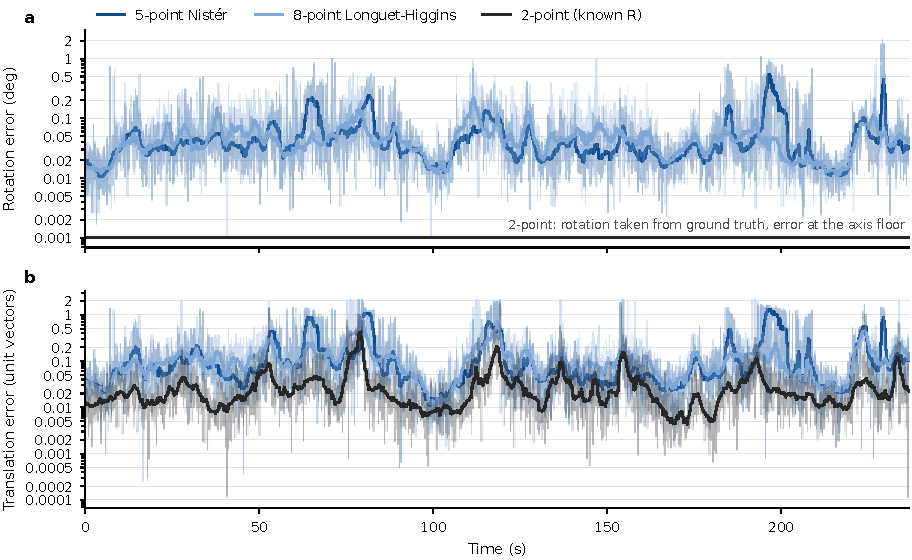
\includegraphics[width=\linewidth]{d4_rpe_time.pdf}
  \caption{Relative pose error of the 2D--2D estimators over the office sequence.
    \textbf{a},~Rotation error. \textbf{b},~Translation-direction error between unit
    vectors. Thin lines show every frame pair; thick lines show a centred 2\,s rolling
    median. RANSAC threshold 0.1\,px, at most 5\,000 iterations, $n = 3\,887$ frame
    pairs per method.}
  \label{fig:d4time}
\end{figure}

\begin{table}[t]
  \centering\small
  \caption{Relative pose error over the full sequence ($n = 3\,887$ frame pairs). Rotation
    is the equivalent angle of the chordal distance; translation is the distance between
    unit direction vectors. Inlier ratio and solver time are per-frame medians. RANSAC
    thresholds are 0.1\,px for the 2D--2D methods and 1\,cm for Arun's method.}
  \label{tab:stats}
  \setlength{\tabcolsep}{4.5pt}
  \begin{tabular}{l rr rrr rr}
    \toprule
    & \multicolumn{2}{c}{Rotation} & \multicolumn{3}{c}{Translation direction}
    & \multicolumn{2}{c}{RANSAC} \\
    \cmidrule(lr){2-3}\cmidrule(lr){4-6}\cmidrule(lr){7-8}
    Method & median & $< 1^\circ$ & median & $< 0.5$ & $< 0.1$ & inliers & time \\
    \midrule
    5-point Nist\'er           & 0.034$^\circ$ & 99.8\,\% & 0.066 & 89.4\,\% & 62.3\,\% & 49\,\% & 85\,ms \\
    8-point Longuet-Higgins    & 0.039$^\circ$ & 99.97\,\% & 0.087 & 95.1\,\% & 55.0\,\% & 45\,\% & 140\,ms \\
    2-point (known $R$)        & ---          & ---       & 0.020 & 99.4\,\% & 92.9\,\% & 48\,\% & 0.39\,ms \\
    3-point Arun (3D--3D)      & 0.019$^\circ$ & 100\,\%  & 0.044 & 98.3\,\% & 82.3\,\% & 41\,\% & 0.25\,ms \\
    \midrule
    5-point, no RANSAC         & 14.0$^\circ$ & 0.3\,\%   & 1.27  & 4.3\,\%  & 0.1\,\% & --- & 6.1\,ms \\
    8-point, no RANSAC         & 1.17$^\circ$ & 42.5\,\%  & 0.77  & 39.1\,\% & 4.9\,\% & --- & 2.0\,ms \\
    Arun, no RANSAC            & 0.61$^\circ$ & 79.5\,\%  & 1.05  & 17.4\,\% & 0.8\,\% & --- & 0.03\,ms \\
    \bottomrule
  \end{tabular}
\end{table}

\paragraph{The inlier threshold sets the accuracy.}
The simulator renders sharp images, and SIFT localises keypoints to a fraction of a
pixel. A threshold far below the usual 1\,px therefore keeps only the most precise
matches, and it improves every estimator (Fig.~\ref{fig:sweep}). Going from 1\,px to
0.1\,px lowers the median translation error of the 5-point solver from 0.59 to 0.063
and its median rotation error from 0.36$^\circ$ to 0.031$^\circ$, while the median
inlier ratio falls from 86\,\% to 48\,\%. The 5-point solver gains the most from the
tighter threshold, and at 0.1\,px it is the more accurate of the two solvers that
estimate rotation and translation together. We use 0.1\,px for all results.

\begin{figure}[t]
  \centering
  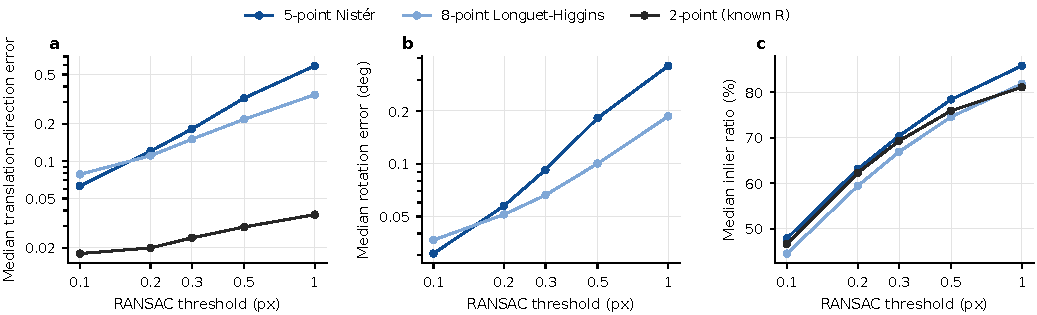
\includegraphics[width=\linewidth]{d4_threshold_sweep.pdf}
  \caption{Effect of the RANSAC inlier threshold, measured on the first 60\,s of the
    sequence ($n \approx 1\,040$ frame pairs per point). \textbf{a},~Median
    translation-direction error. \textbf{b},~Median rotation error of the 5- and 8-point
    solvers (the 2-point solver takes the rotation as input). \textbf{c},~Median inlier
    ratio.}
  \label{fig:sweep}
\end{figure}

\paragraph{Known rotation.}
Given the rotation, the 2-point solver has a median translation error of 0.020, three
times lower than the 5-point solver, and 92.9\,\% of its frame pairs are below 0.1.
Its rotation error is zero up to floating point because the rotation is taken from
ground truth; on a real drone it would come from the gyroscope, and the gyroscope
error would add to it. The solver is also more than 200 times faster than the
5-point solver (0.39\,ms against 85\,ms per frame), because each hypothesis costs two
cross products and RANSAC needs far fewer samples.

\paragraph{Pose publication.}
For every frame pair the node publishes the estimate on \code{/camera\_pose}, chained
onto the previous ground-truth pose (Section~\ref{sec:impl}), and the ground truth on
\code{/gt\_camera\_pose}. RViz shows both for any estimator selected with the
\code{pose\_estimator} flag.

\subsection{3D--3D registration with Arun's method (Deliverable 5)}\label{sec:d5}

With the depth image, each match becomes a pair of 3D points and the relative pose is
the rigid transform between two point clouds. Three points determine it, and Arun's
SVD solution~\cite{arun1987least} gives it in closed form. Depth also fixes the metric
scale, which no 2D--2D method observes. Arun's method has the lowest rotation error
of the estimators that solve for rotation, a median of 0.019$^\circ$, and every frame pair stays below
1$^\circ$ (Fig.~\ref{fig:d5time}, Table~\ref{tab:stats}). The median metric translation
error is 1.7\,mm for a median step of 31\,mm. A threshold sweep on the first 60\,s gives
the same rotation accuracy for thresholds between 0.5 and 2\,cm (0.016--0.017$^\circ$);
at 10\,cm the median rotation error rises to 0.031$^\circ$ and the translation error to
3.4\,mm. We use 1\,cm. With a minimal set of three, RANSAC is cheap, and the whole
estimate takes 0.25\,ms per frame.

\begin{figure}[t]
  \centering
  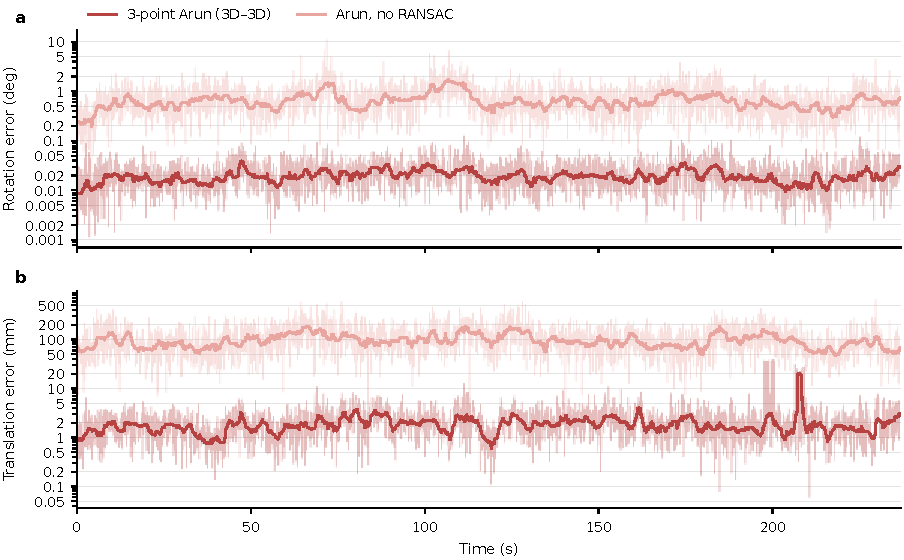
\includegraphics[width=\linewidth]{d5_arun_rpe_time.pdf}
  \caption{Relative pose error of Arun's 3D--3D method over the office sequence, with
    RANSAC (1\,cm threshold) and fitted to all matches without RANSAC.
    \textbf{a},~Rotation error. \textbf{b},~Metric translation error. Thin lines show
    every frame pair; thick lines show a centred 2\,s rolling median; $n = 3\,887$.}
  \label{fig:d5time}
\end{figure}

\subsection{What RANSAC contributes (optional baselines)}\label{sec:noransac}

Fig.~\ref{fig:cdf} places all seven estimators on common axes. Fitting a model to every
ratio-test match, outliers included, moves the error distribution by one to two orders
of magnitude. The 5-point solver without RANSAC fits Nist\'er's polynomial system to
all matches and keeps the solution that places the most points in front of both
cameras; its median rotation error reaches 14$^\circ$. The least-squares 8-point and Arun fits degrade more gracefully,
with median rotation errors of 1.2$^\circ$ and 0.6$^\circ$, but their translation
directions are close to random (medians of 0.77 and 1.05 on a scale of 0 to 2). With
RANSAC, the same matches give rotation errors below 0.1$^\circ$ for more than 80\,\% of
frame pairs with every solver. The ordering of the RANSAC curves also shows the value
of prior information: the 2-point solver, which knows the rotation, and Arun's method,
which knows the depth, both lie to the left of the 5- and 8-point solvers in
translation.

\begin{figure}[t]
  \centering
  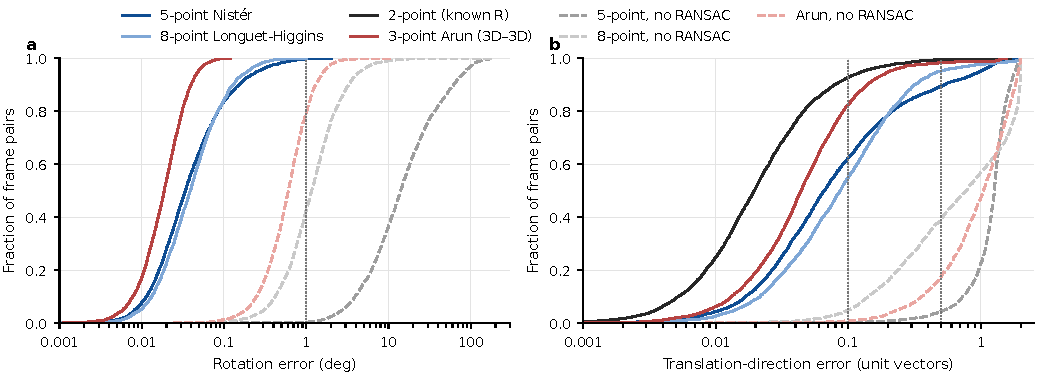
\includegraphics[width=\linewidth]{d4_d5_error_cdf.pdf}
  \caption{Empirical cumulative distributions of the relative pose error for all
    estimators over the full sequence ($n = 3\,887$ frame pairs each). Solid lines use
    RANSAC; dashed lines fit all matches at once. \textbf{a},~Rotation error; the
    2-point solver is omitted because its rotation is given. \textbf{b},~Translation-direction
    error. Dotted lines mark 1$^\circ$, 0.1 and 0.5.}
  \label{fig:cdf}
\end{figure}


\FloatBarrier
\renewcommand{\bibfont}{\small}
\setlength{\bibsep}{2pt}
\bibliographystyle{unsrtnat}
\bibliography{references}

\end{document}
